\documentclass{article}
\usepackage[margin=1in]{geometry}
\usepackage{microtype}
\usepackage{setspace}
\usepackage{amsmath}
\usepackage{parskip}
\usepackage{amssymb}
\usepackage{graphicx}

\graphicspath{{../public/}}

\parskip=4ex
\date{}
\author{}

\title{12.8 Change of Variables in Multiple Integrals}

\begin{document}
  \maketitle
  In one dimensional calculus, change of variable (substitution) is often used to simplfy an integral. By reversing the roles of $ x ~\&~ u$, the Substitution Rule can be written as
  \[
    \int^{b}_{a} f(x)~dx = \int^{d}_{c} f(g(u))g'(u)~du
  \]

  where $ x=g(u), a=g(c), ~\&~ b=g(d) $. Another way to express the Substitution Rule is
  \[
    \int^{b}_{a} f(x)~dx = \int^{d}_{c} f(x(u))~\frac{dx}{gu}du
    n
  \]

  A change of variables is also useful in double integrals, an example would be conversion to polar coordinates. Where the new variables $ r ~\&~ \theta $ are related to the old variables $ x ~\&~ y $ by the equations
  \[
    x=r\cos{\theta} \qquad y=r\sin{\theta}
  \]

  The change of variables formula can be written as
  \[
    \INT*{^{},_E} f(x,y)~dA = \INT*{^{},_S} f(r\cos{\theta}, r\sin{\theta})r~drd\theta
  \]

  where $ S $ is the region in the $ r\theta $ plane that corresponds to the region $ R $ in the $ xy $ plane.

  Consider a change of variables that is given by a transformation $ T $ from the $ uv $ plane to the $ xy $ plane
  \[
    T(u,v)=(x,y)
  \]

  where $ x ~\&~ y $ are related to $ u ~\&~ v $ by the equations
  \[
    x=g(u,v) \qquad y=h(u,v)
  \]

  or alternatively
  \[
    x=x(u,v) \qquad y=y(u,v)
  \]

  It is usually assumed that $ T $ is a $ C^{1} $ transformation, meaning that $ g ~\&~ h $ have continuous first-order partial derivatives.
  
  $ T $ is a function whose domain and range are both subsets of $ \mathbb{R}^{2} $. If $ T(u_1,v_1)=(x_1,y_1) $, then the point $ (x_1,y_1) $ is known as the image of the point $ (u_1,v_1) $. $ T $ is called one-to-one if no two points have the same image.

  \begin{center}
    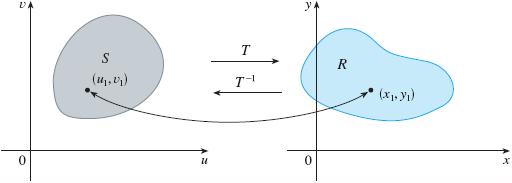
\includegraphics[width=8cm]{12_8_1}
  \end{center}

  The figure above shows the effect of a transformation $ T $ on a region $ S $ in the $ uv $ plane. $ T $ transforms $ S $ into a region $ R $ in the $ xy $ plane called the image of $ S $. The region $ R $ consists of images of all points in $ S $.

  The inverse transformation $ T^{-1} $ exists if $ T $ is one-to-one. To clarify, $ T^{-1} $ is the transformation from the $ xy $ plane to the $ uv $ plane and it may be possible to solve for $ u ~\&~ v $ in terms of $ x ~\&~ y $ in terms of the equations below 
  \[
    x=g(u,v) \qquad y=h(u,v)
  \]

  So
  \[
    u=G(x,y) \qquad v=H(x,y)
  \]

  \textbf{Ex 1}
  \[
    x=u^{2}-v^{2} \qquad y=2uv
  \]

  Find the image of the square $ S=\{ (u,v) \bigg| 0 \le u \le 1, 0 \le v \le 1 \} $ 
  \[
    \begin{gathered}
    S_1, v=0~(0 \le u \le 1)\\
    x=u^{2} \qquad y=2u(0)=0,~(0 \le x \le 1)\\
    ~\\
    S_2, u=0~(0 \le v \le 1)\\
    x=-v^{2} \qquad y=2(0)v=0 ~ (-1 \le x \le  0)\\
    ~\\
    S_3, v=1~(0 \le u \le 1)\\
    x=u^{2}-1 \qquad y = 2u(1)=2u \to u= \frac{y}{2} \qquad x=\frac{y^{2}}{4}-1 ~ (-1 \le x \le 0)\\
    ~\\
    S_4, u=1 ~ (0 \le v \le 1)\\
    x=1-v^{2} \qquad y=2(1)v =2v \to v=\frac{y}{2} \qquad x=1-\frac{y^{2}}{4} ~ (0 \le x \le 1)\\
    \end{gathered}
  \]

  So we have $ y=0 ~(0 \le x \le 1), y=0~(-1 \le x \le 0), x=\frac{y^{2}}{4}-1~(-1 \le x \le 0),x=1-\frac{y^{2}}{4}~(0 \le x \le 1) $, giving us the image of $ S $ which we call $ R $.   

  \begin{center}
    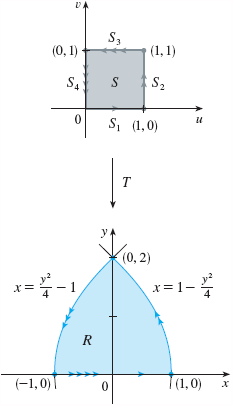
\includegraphics[width=5cm]{12_8_2}
  \end{center} 

  \textbf{Effects of Change of Variable on Double Integrals}\\
  A small rectangle $ S $ in the $ uv $ plane whose lower left corner is the point $ (u_0,v_0) $ and whose dimensions are $ \Delta u ~\&~  \Delta v $, shown in the figure below

  \begin{center}
    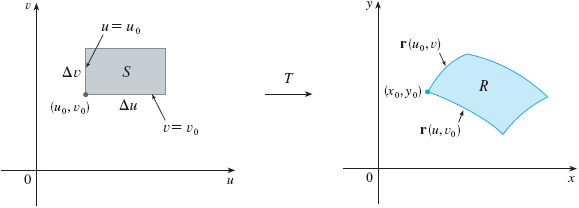
\includegraphics[width=10cm]{12_8_3}
  \end{center}

  The image of $ S $ is a region $ R $ in the $ xy $ plane, one of whose boundary points is $ x_0,y_0 =T(u_0,v_0) $. The vector
  \[
    r(u,v) = g(u,v)i+ h(u,v)j
  \]

  is the position vector of the image of the point $ (u,v) $. The equation representing the lower side of $ S $  is $ v=v_0 $, whose image curve is given by the vector function $ r(u,v_0) $. The tangent vector at $ x_0,y_0 $ to this image curve is
  \[
    r_u= g_u(u_0,v_0)i + h_u(u_0,v_0)j = \frac{\partial x}{\partial u}i + \frac{\partial y}{\partial eqRu}
  \]

  While the tangent vector at $ x_0,y_0 $ to the image curve of the left side of $ S $, namely $ u=u_0 $ is
  \[
    r_v = g_v(u_0, v_0)i + h_v(u_0, v_0)j = \frac{\partial x}{\partial v} + \frac{\partial y}{\partial v}eqj
  \]

  The image region $ R=T(S) $ can be approximated by the secant vectors
  \[
    a=r(u_0+ \Delta u,v_0) - r(u_0,v_0) \qquad b=r(u_0,v_0 + \Delta v) - r(u_0,v_0)
  \]

  demonstrated in the diagram below
  \begin{center}
    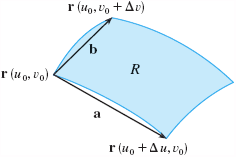
\includegraphics[width=6cm]{12_8_4}
  \end{center}

  But
  \[
    r_u = \lim_{\Delta u \to 0}{\frac{r(u_0+ \Delta u, v_0) - r(u_0,v_0)}{\Delta u}}
  \]

  and so 
  \[
    r(u_0+\Delta u, v_0) - r(u_0,v_0) \approx \Delta u r_u
  \]

  Similarly
  \[
    r(u_0, v_0 = \Delta v) - r(u_0,v_0) \approx \Delta u r_v
  \]

  Meaning $ R $ can be approximated by a paralellogram determined by the vectors $ \Delta u r_u ~\&~ \Delta vr_v $ (see figure below).
  \begin{center}
    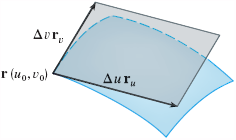
\includegraphics[width=6cm]{12_8_5}
  \end{center}

  Therefore the area of $ R $ can be approximated by the area of this paralleloogram,
  \[
    \bigg| (\Delta u r_u) \times (\Delta v r_v) \bigg| = \bigg| r_u \times r_v \bigg| \Delta u \Delta v
  \]

  Computing the cross product gives
  \[
    r_u \times r_v = 
    \begin{vmatrix}
    i &j &k\\
    \frac{\partial x}{\partial u} &\frac{\partial y}{\partial u} &0\\
    \frac{\partial x}{\partial v} &\frac{\partial y}{\partial v} &0
    \end{vmatrix} =
    \begin{vmatrix}
    \frac{\partial x}{\partial u} &\frac{\partial y}{\partial u}\\
    \frac{\partial x}{\partial v} &\frac{\partial y}{\partial v}
    \end{vmatrix}k =
    \begin{vmatrix}
    \frac{\partial x}{\partial u} &\frac{\partial x}{\partial v}\\
    \frac{\partial y}{\partial u} &\frac{\partial y}{\partial v}
    \end{vmatrix}k
  \]

  This determinant is called the Jacobian of the transformation and has a special notation
  
  \textbf{Definition}\\
  The Jacobian of the transformation $ T $ given by $ x=g(u,v) ~\&~ y=h(u,v) $ is
  \[
    \frac{\partial (x,y)}{\partial (u,v)} = 
    \begin{vmatrix}
    \frac{\partial x}{\partial u} &\frac{\partial x}{\partial v}\\
    \frac{\partial y}{\partial u} &\frac{\partial y}{\partial v}
    \end{vmatrix} = \frac{\partial x}{\partial u}\frac{\partial y}{\partial v}-\frac{\partial x}{\partial v}\frac{\partial y}{\partial u}
  \]

  With this notation, $ r(u_0, v_0 = \Delta v) - r(u_0,v_0) \approx \Delta u r_v $ can be used to give an approximation to the area $ \Delta A $ of $ R $:
  \[
    \Delta A \approx \bigg| \frac{\partial (x,y)}{\partial (u,v)} \bigg| \Delta u \Delta v
  \]

  where the Jacobian is evaluated at $ (u_0, v_0) $ 
  
  Next, $ S $ in the $ uv $ plane is divided into rectangles $ S_{ij} $ and their images in the $ xy $ plane is known as $ R_{ij} $.

  By approximating to each $ R_{ij} $, the double integral of $ f $ over $ R $ is
  \[
    \begin{gathered}
    \INT*{^{},_R} f(x,y)~dA \approx \sum^{m}_{i=1}  \sum^{n}_{j=1} f(x_i,y_j)~ \Delta A\\
    \sum^{m}_{i=1}  \sum^{n}_{j=1} f(g(u_i), h(u_i,v_j)) \bigg| \frac{\partial (x,y)}{\partial (u,v)} \bigg| \Delta u \Delta v 
    \end{gathered}
  \]

  where the Jacobian is evaluated at $ (u_i, v)j $. We can see this double sum is a Riemann sum for the integral
  \[
    \INT*{^{},_S} f(g(u,v), h(u,v)) \bigg| \frac{\partial (x,y)}{\partial (u,v)} \bigg| ~dudv
  \]
  
  \textbf{Theorem 9)Change of Variables in a Double Integral}\\
  Suppouse $ T $, a $ C^{1} $ transformation, whose Jacobian is nonzero and maps a region $ S $ in the $ uv $ plane onto a region $ R $ in the $ xy $ plane. Suppouse that $ f $ is continuous on $ R $ and that $ R ~\&~ S $ are Type I or Type II plane regions. Suppouse that $ T $ is one-to-one, except perhaps on S's boundaries. Then
  \[
    \INT*{^{},_R} f(x,y)~dA = \INT*{^{},_S} f(x(u,v), y(u,v)) \bigg| \frac{\partial (x,y)}{\partial (u,v)} \bigg| ~ dudv
  \]
  
  Meaning that we change from an integral in $ x ~\&~ y $ to an integral in $ u ~\&~ v $ by expressing $ x ~\&~ y $ as functions of $ u ~\&~ v $ and writing
  \[
    dA = \bigg| \frac{\partial (x,y)}{\partial (u,v)} \bigg|~dudv
  \]

  The transformation $ T $ from the $ r\theta $ to the $ xy $ plane is given by
  \[
    x = g(r,\theta)= r\cos{\theta} \qquad y=h(r,\theta) = r\sin{\theta}
  \]

  The geometry of the transformation is shown below. $ T $ maps a rectangle in the $ r\theta $ plane to a polar rectangle in the $ xy $ plane. The Jacobian of $ T $ is
  \[
    \frac{\partial (x,y)}{\partial (u,v)} =
    \begin{vmatrix}
    \frac{\partial x}{\partial r} &\frac{\partial x}{\partial \theta}\\
    \frac{\partial y}{\partial r} &\frac{\partial y}{\partial \theta}=
    \begin{vmatrix}
    \cos{\theta} &-r\sin{\theta}\\
    \sin{\theta} &r\cos{\theta}
    \end{vmatrix} =
    r\cos^{2}{\theta} + r\sin^{2}{\theta}=r>0
    \end{vmatrix}
  \]
  
  \begin{center}
    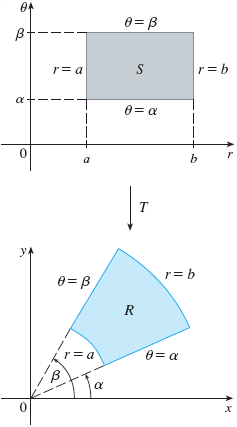
\includegraphics[width=6cm]{12_8_6}
  \end{center}

  So Theorem 9 gives
  \[
    \begin{gathered}
      \INT*{^{},_R} f(x,y)~dxdy = \INT*{^{},_S} f(r\cos{\theta}, r\sin{\theta}) 
      \bigg| \frac{\partial (x,y)}{\partial (r,\theta)} \bigg|~drd\theta\\
      \int^{\alpha}_{\beta} \int^{b}_{a} f(r\cos{\theta}, r\sin{\theta})r ~drd\theta 
    \end{gathered}
  \]

  \textbf{Ex 2}\\
  Use the change of variables $ x=u^{2}-v^{2} ~\&~ y=2uv $ to evaluate the integral $ \INT*{^{},_R} y~dA$, where $ R $ is the region bounded by the $ x $ axis and the parabolas $ y^{2}=4-4x ~\&~ y^{2}=4x, y \ge 0 $.  

  Previously, we worked with $ x=u^{2}-v^{2} ~\&~ y=2uv $ and $ T(S)=R $, where $ S $ is the square $ \bigg| 0,1 \bigg| \times \bigg| 0,1 \bigg| $. Evaluating the integral for $ S $ is much simpler than for $ R $. First, compute the jacobian
  \[
    \begin{gathered}
    \frac{\partial (x,y)}{\partial (u,v)}=
    \begin{vmatrix}
    \frac{\partial x}{\partial u} &\frac{\partial x}{\partial v}\\
    \frac{\partial y}{\partial u} &\frac{\partial y}{\partial v}
    \end{vmatrix}=
    \begin{vmatrix}
    2u &-2v\\
    2v &2u
    \end{vmatrix}=
    4u^{2}+4v^{2} > 0
    \end{gathered}
  \]

  So
  \[
    \INT*{^{},_R}y~dA = \INT*{^{},_S} 2uv \bigg| \frac{\partial (x,y)}{\partial (u,v)} \bigg|~dA = \int^{1}_{0} \int^{1}_{0} (2uv)4(u^{2}+v^{2}) ~ dudv = \boxed{2}
  \]
  
  \textbf{Ex 3}\\
  Evaluate the integral $ \INT*{^{},_R} e^{\frac{x+y}{x-y}}$, where $ R $ is the trapezoidal region with vertices $ (1,0),(2,0),(0,-2), ~\&~ (0,-1) $.

  \[
    u=x+y \qquad v=x-y
  \]

  We then solve for $ x ~\&~ y $
  \[
    \begin{gathered}
    u+v=(x+y)+(x-y)\\
    2x=u+v\\
    x=\frac{1}{2}(u+v)\\
    ~\\
    u-v=(x+y)-(x-y)\\
    2y=u-v\\
    y=\frac{1}{2}(u-v)
    \end{gathered}
  \]

  Now compute the Jacobian
  \[
    \begin{gathered}
    \frac{\partial (x,y)}{\partial (u,v)}=
    \begin{vmatrix}
    \frac{\partial x}{\partial u} &\frac{\partial x}{\partial v}\\
    \frac{\partial y}{\partial u} &\frac{\partial y}{\partial v}
    \end{vmatrix}=
    \begin{vmatrix}
    \frac{1}{2} &\frac{1}{2}\\
    \frac{1}{2} &-\frac{1}{2}
    \end{vmatrix}=
    -\frac{1}{2}
    \end{gathered}
  \]

  The sides of $ R $ lie on the lines
  \[
    y=0 \qquad x-y = 2 \qquad x=0 \qquad x-y=1
  \]

  By using the equations $ x ~\&~ y $ that are in terms of $ u ~\&~ v $, we obtain
  \[
    u=v \qquad v=2 \qquad u=-v \qquad v=1
  \]

  So
  \[
    S=\{ (u,v) \bigg| 1 \le v \le 2, -v \le u \le v \}
  \]
  
  Which gives
  \[
    \begin{gathered}
      \INT*{^{},_R}e^{\frac{x+y}{x-y}}~dA=\INT*{^{},_S}e^{\frac{u}{v}} \bigg| \frac{\partial (x,y)}{\partial (u,v)} \bigg|~dudv\\
      \int^{2}_{1} \int^{v}_{-v} e^{\frac{u}{v}}\frac{1}{2} ~ dudv =\boxed{\frac{3}{4}(e-e^{-1})}
    \end{gathered}
  \]

  \textbf{Triple Integrals}\\
  Let $ T $ be a transformation that maps a region $ S $ in $ uvw $ space onto a region $ R $ in $ xyz $ space by means of the equations
  \[
    x=g(u,v,w) \qquad y=h(u,v,w) \qquad z=k(u,v,w)
  \]

  The Jacobian of $ T $ is the $ 3 \times 3 $ determinant
  \[
   \frac{\partial (x,y,z)}{\partial (u,v,w)} =
   \begin{vmatrix}
   \frac{\partial x}{\partial u} &\frac{\partial x}{\partial v} &\frac{\partial x}{\partial w}\\
   \frac{\partial y}{\partial u} &\frac{\partial y}{\partial v} &\frac{\partial y}{\partial w}\\
   \frac{\partial z}{\partial u} &\frac{\partial z}{\partial v} &\frac{\partial z}{\partial w}
   \end{vmatrix}
  \]

  \[
    \begin{gathered}
    \INT*{^{},_R,^{}}f(x,y,z)~dV\\
    \to\\
    \INT*{^{},_S,^{}} f(x(u,v,w),y(u,v,w),z(u,v,w))
    \bigg| \frac{\partial (x,y,z)}{\partial (u,v,w)} \bigg|~dudvdw
    \end{gathered}
  \]

  \textbf{Ex 4}\\
  Derive the formula for triple integration in spherical coordinates
  \[
    x=\rho \sin{\phi}\cos{\theta} \qquad y=\rho\sin{\phi}\sin{\theta} \qquad z=\rho\cos{\phi}
  \]

  Compute the Jacobian
  \[
    \begin{gathered}
    \frac{\partial (x,y,z)}{\partial (\rho,\theta, \phi)}=
    \begin{vmatrix}
    \sin{\phi}\cos{\theta} &-\rho\sin{\phi}\sin{\theta} &\rho\cos{\phi}\cos{\theta}\\
    \sin{\phi}\sin{\theta} &\rho\sin{\phi}\cos{\theta} &\rho\cos{\phi}\sin{\theta}\\
    \cos{\phi} &0 &-\rho\sin{\phi}
    \end{vmatrix} = -rho^{2}\sin{\phi}
    \end{gathered}
  \]

  Since $ 0 \le \phi \le \pi $, $ \sin{\phi} \ge 0 $. Therefore
  \[
    \begin{gathered}
    \bigg| \frac{\partial (x,y,z)}{\partial (\rho,\theta,\phi)} \bigg| = \rho^{2}\sin{\phi}\\
    ~\\
    \INT*{^{},_R,^{}}f(x,y,z)~dV\\
    \to\\
    \boxed{\INT*{^{},_S,^{}}f(\rho\sin{\phi}\cos{\theta},\rho\sin{\phi}\sin{\theta},\rho\cos{\phi})\rho^{2}\sin{\phi} ~d\rho d\theta d\phi}
    \end{gathered}
  \]
  
  
  
  
  
  
  
  


  
  
  
  
  
\end{document}
